\documentclass{beamer}
\usepackage[utf8]{inputenc}
\setbeamertemplate{navigation symbols}{}

\usetheme{Madrid}
\usecolortheme{default}


%------------------------------------------------------------
%This block of code defines the information to appear in the
%Title page
\title[Missing Pollution Data] %optional
{Filling in the Gaps: Using Consumer Products to Replace Missing Pollution Data}

% \subtitle{A short story}

\author[Watt, Aaron] % (optional)
{A.~C.~Watt\inst{1}}

\institute[UCB] % (optional)
{
  \inst{1}%
  Agricultural \& Resource Economics\\
  University of California, Berkeley
}

\date[SYP 2022] % (optional)
{Second Year Paper, March 2022}

%---------------------------------------------------------



%---------------------------------------------------------
% Introduction

\AtBeginSection[]
{
  \begin{frame}
    \frametitle{Table of Contents}
    \tableofcontents[currentsection]
  \end{frame}
}
%------------------------------------------------------------


\begin{document}

%The next statement creates the title page.
\frame{\titlepage}


%---------------------------------------------------------
%This block of code is for the table of contents after
%the title page
\begin{frame}
\frametitle{Motivation}
\textbf{Clean Air} 

\begin{itemize}
    \item The Clean Air Act (1970) established National Ambient Air Quality Standards
    (NAAQS) for US counties
    \item Either "attainment" or "non-attainment", penalties/forced adoption
    \item Minimum requirement of 75\% of readings, per quarter
    \item Air quality can change quickly
    \item Monitor shutoffs are common
\end{itemize}
\vspace{2em}
\textbf{Research Questions}
\begin{itemize}
\item How biased are EPA monitor-based measures of local air quality?
\item Does this bias significantly change NAAQS attainment status?
\end{itemize}

\end{frame}
%---------------------------------------------------------



%---------------------------------------------------------
\begin{frame}
\frametitle{EPA National Ambient Air Quality Standards Monitors}

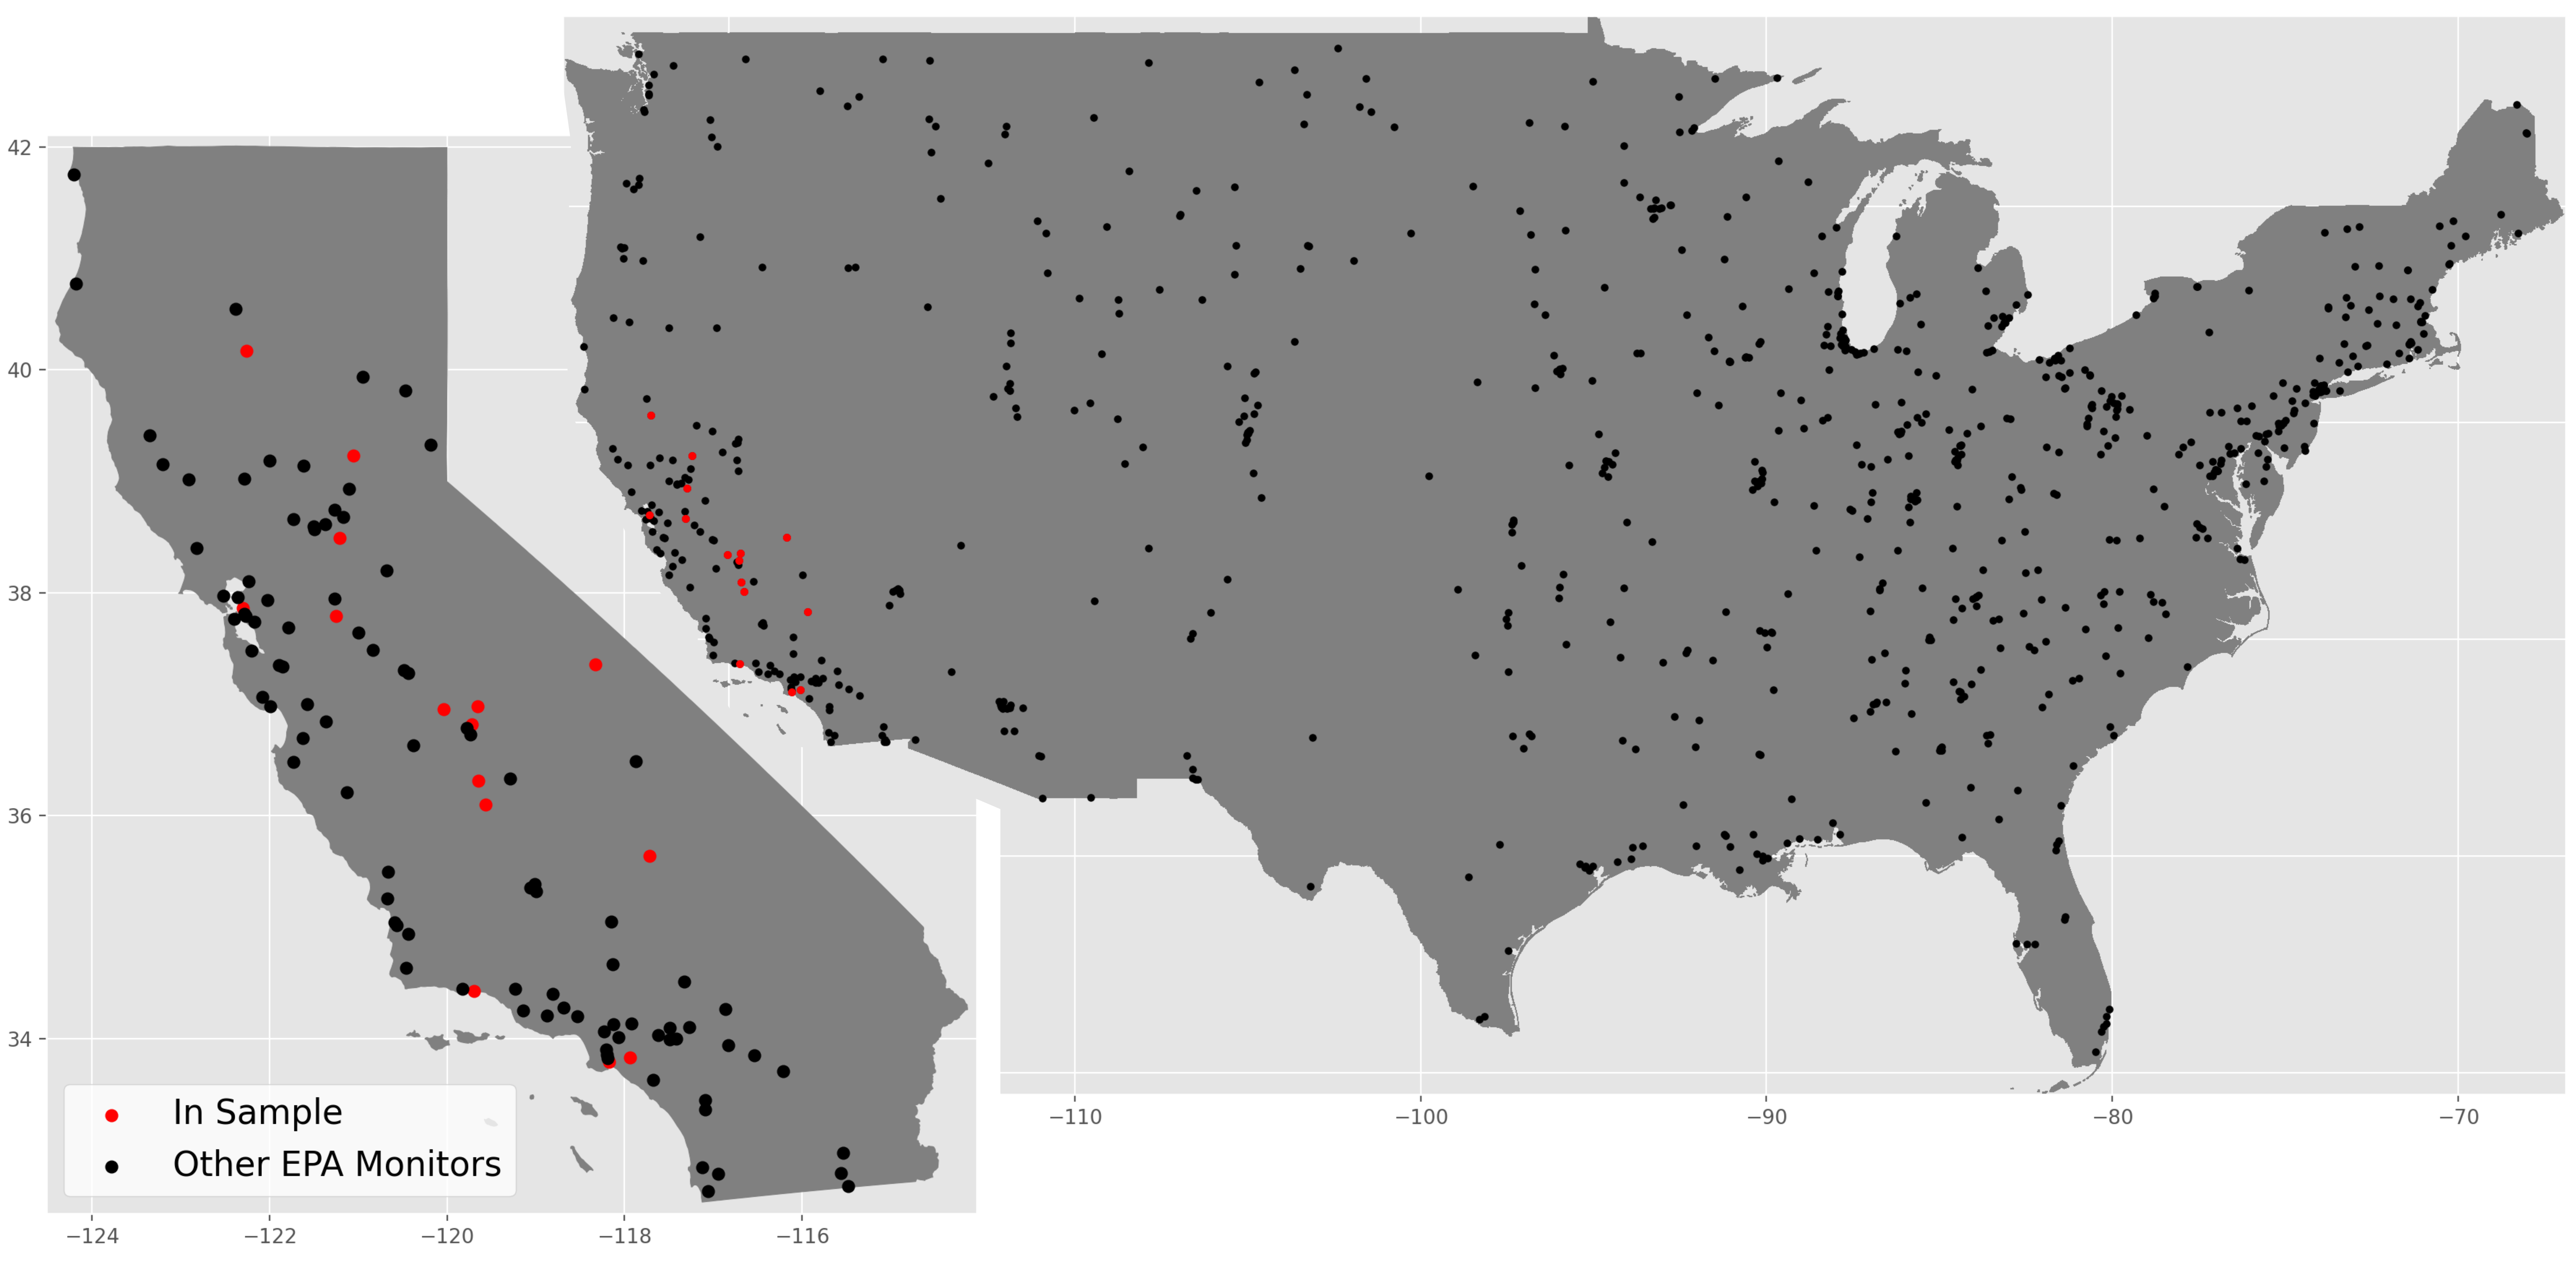
\includegraphics[width=\textwidth]{output/figures/epa/combined_uc_cali_epa.png}
\end{frame}

%---------------------------------------------------------


%---------------------------------------------------------
%Example of the \pause command
\begin{frame}
\frametitle{National Ambient Air Quality Standards for PM2.5}
Two standards for assessing compliance for ambient PM2.5 concentrations at the location of a monitor:
\vspace{2em}

\textbf{Daily Design Value} (average)
\begin{itemize}
    \item[$\Rightarrow$] 3-year rolling average of 1-year average of daily averages
    \item[$\Rightarrow$] standard currently set at 15.0 $\mu$g/m$^3$
\end{itemize}
\vspace{1em}

\textbf{24-Hour Design Value} (98$^{th}$ percentile)
\begin{itemize}
    \item[$\Rightarrow$] 3-year rolling average of 1-year 98$^{th}$ percentile of daily averages
    \item[$\Rightarrow$] standard currently set at 35 $\mu$g/m$^3$
\end{itemize}
\end{frame}
%---------------------------------------------------------


%---------------------------------------------------------
%Highlighting text
\begin{frame}
\frametitle{NAAQS Completeness Criteria for daily monitors}

\textbf{Valid day:}
minimum of 75\% hours reported  (18 hours)

\vspace{2em}
\textbf{Valid quarter:}
minimum of 75\% valid days  (22-23 days\footnote{fewer for monitors that report less frequent observations})

\vspace{2em}
\textbf{Valid quarterly design value:}
all 12 quarters in 3-year period (12 quarters)

\end{frame}
%---------------------------------------------------------


%---------------------------------------------------------
%Observed EPA Completeness
\begin{frame}
\frametitle{Observed Completeness of NAAQS Monitors in sample}
\includegraphics[width=0.8\textwidth]{example-image-a}
\end{frame}
%---------------------------------------------------------


%---------------------------------------------------------
%Purple Air Outdoor Monitors
\begin{frame}
\frametitle{PurpleAir Outdoor Monitors}
\hspace{1em}
PurpleAir Sensors in California 
\hspace{4em}
LA Site Example \\

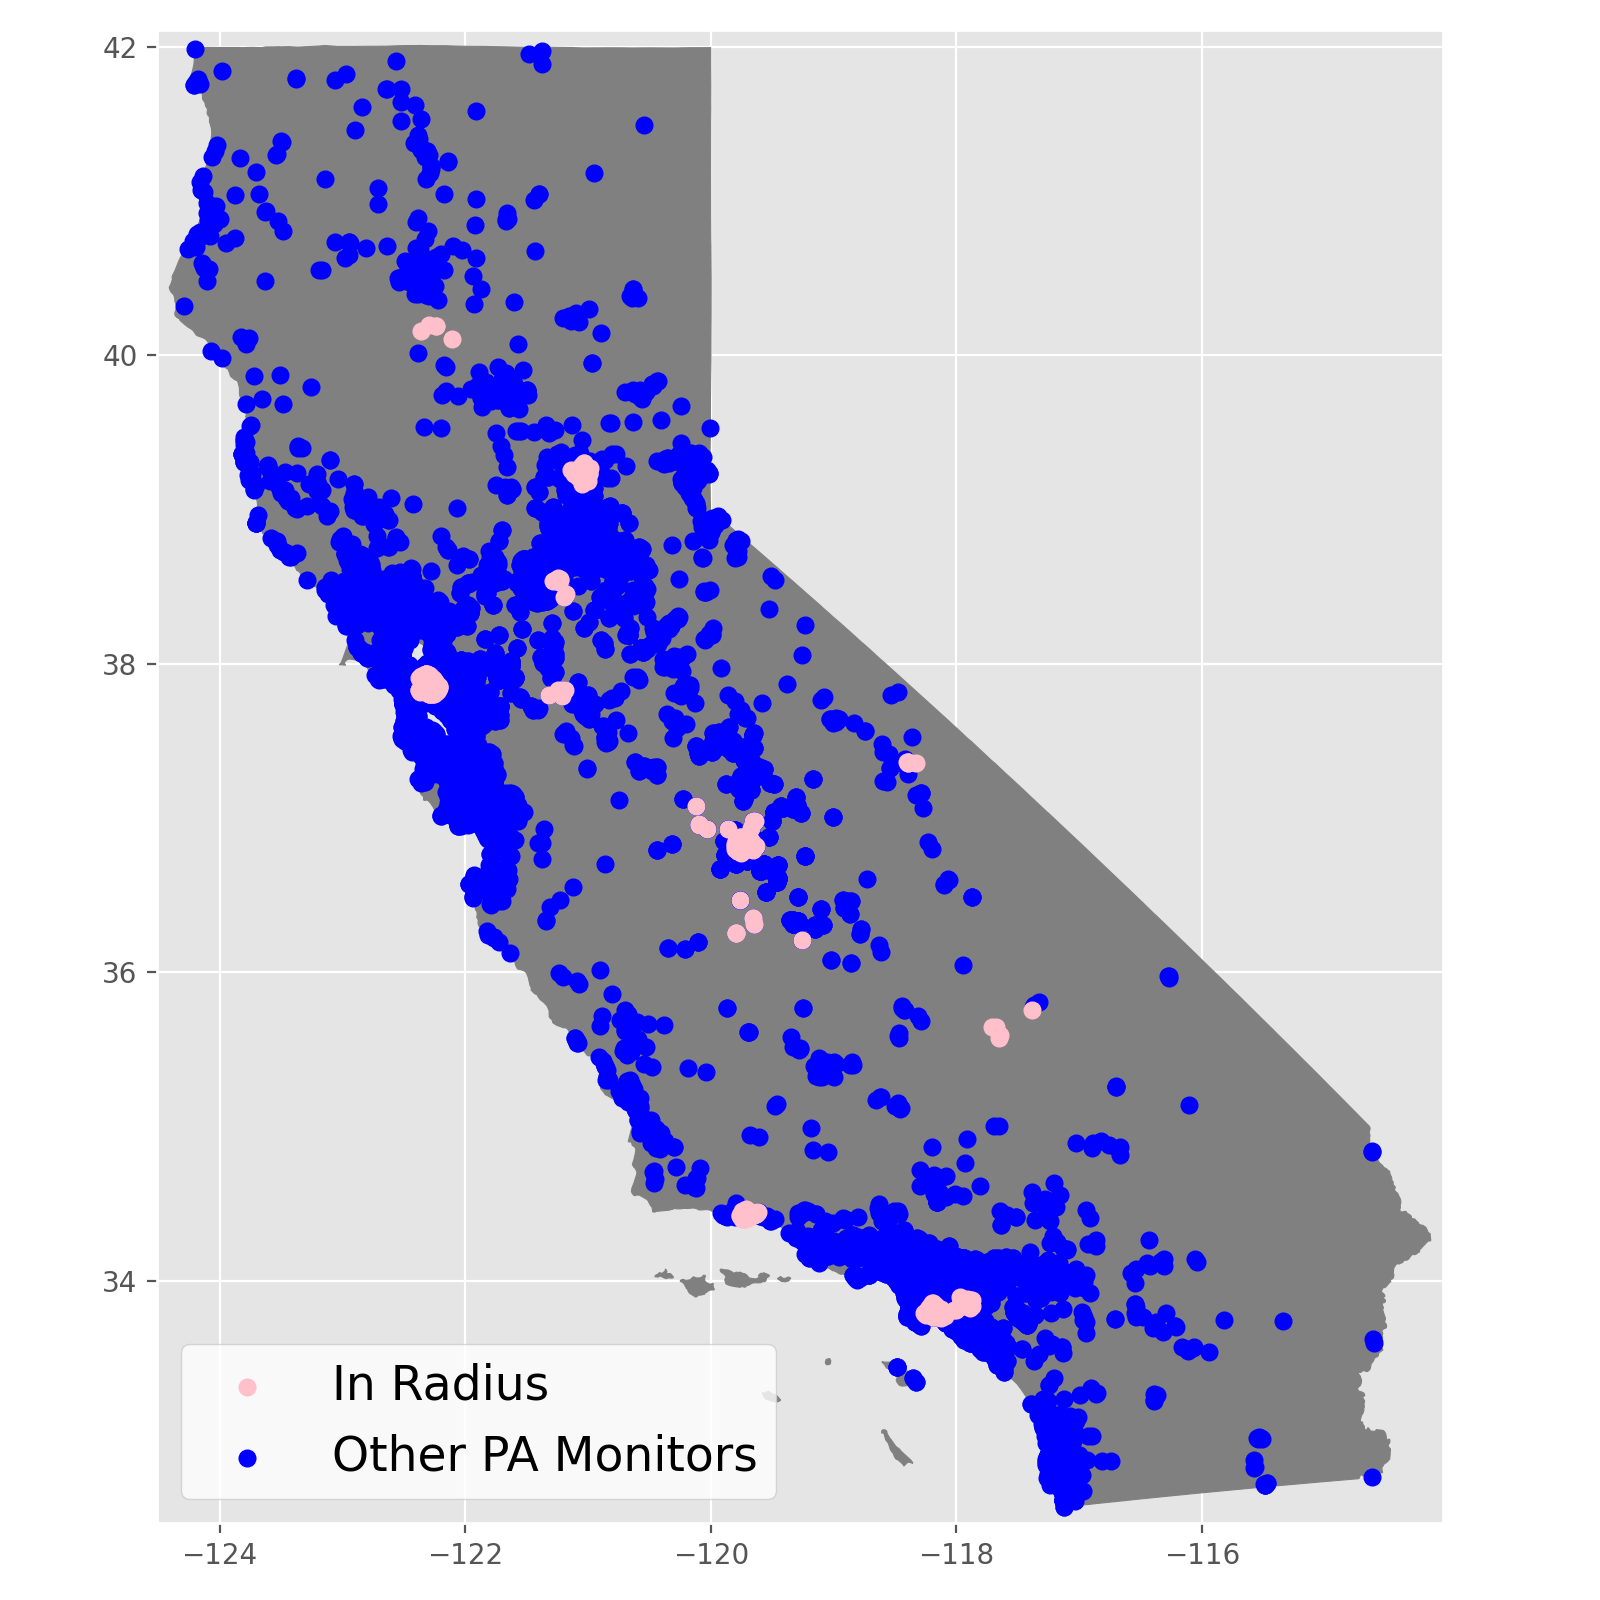
\includegraphics[width=0.49\textwidth]{output/figures/pa/all_ca_and_15_pa_monitors.png}
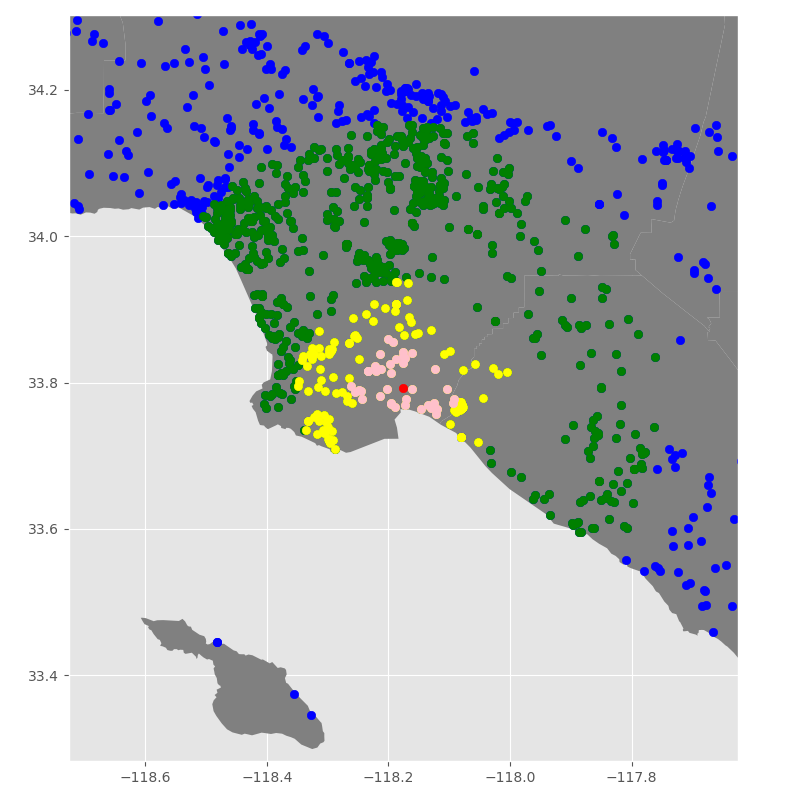
\includegraphics[width=0.49\textwidth]{output/figures/concentric_ranges/county-037_site-4004_epa-pa-concentric-ranges.png}
\end{frame}
%---------------------------------------------------------


%---------------------------------------------------------
%Alternate measure of ambient air quality
\begin{frame}
\frametitle{Alternate measure of ambient PM2.5 Concentration}

\hspace{7em}
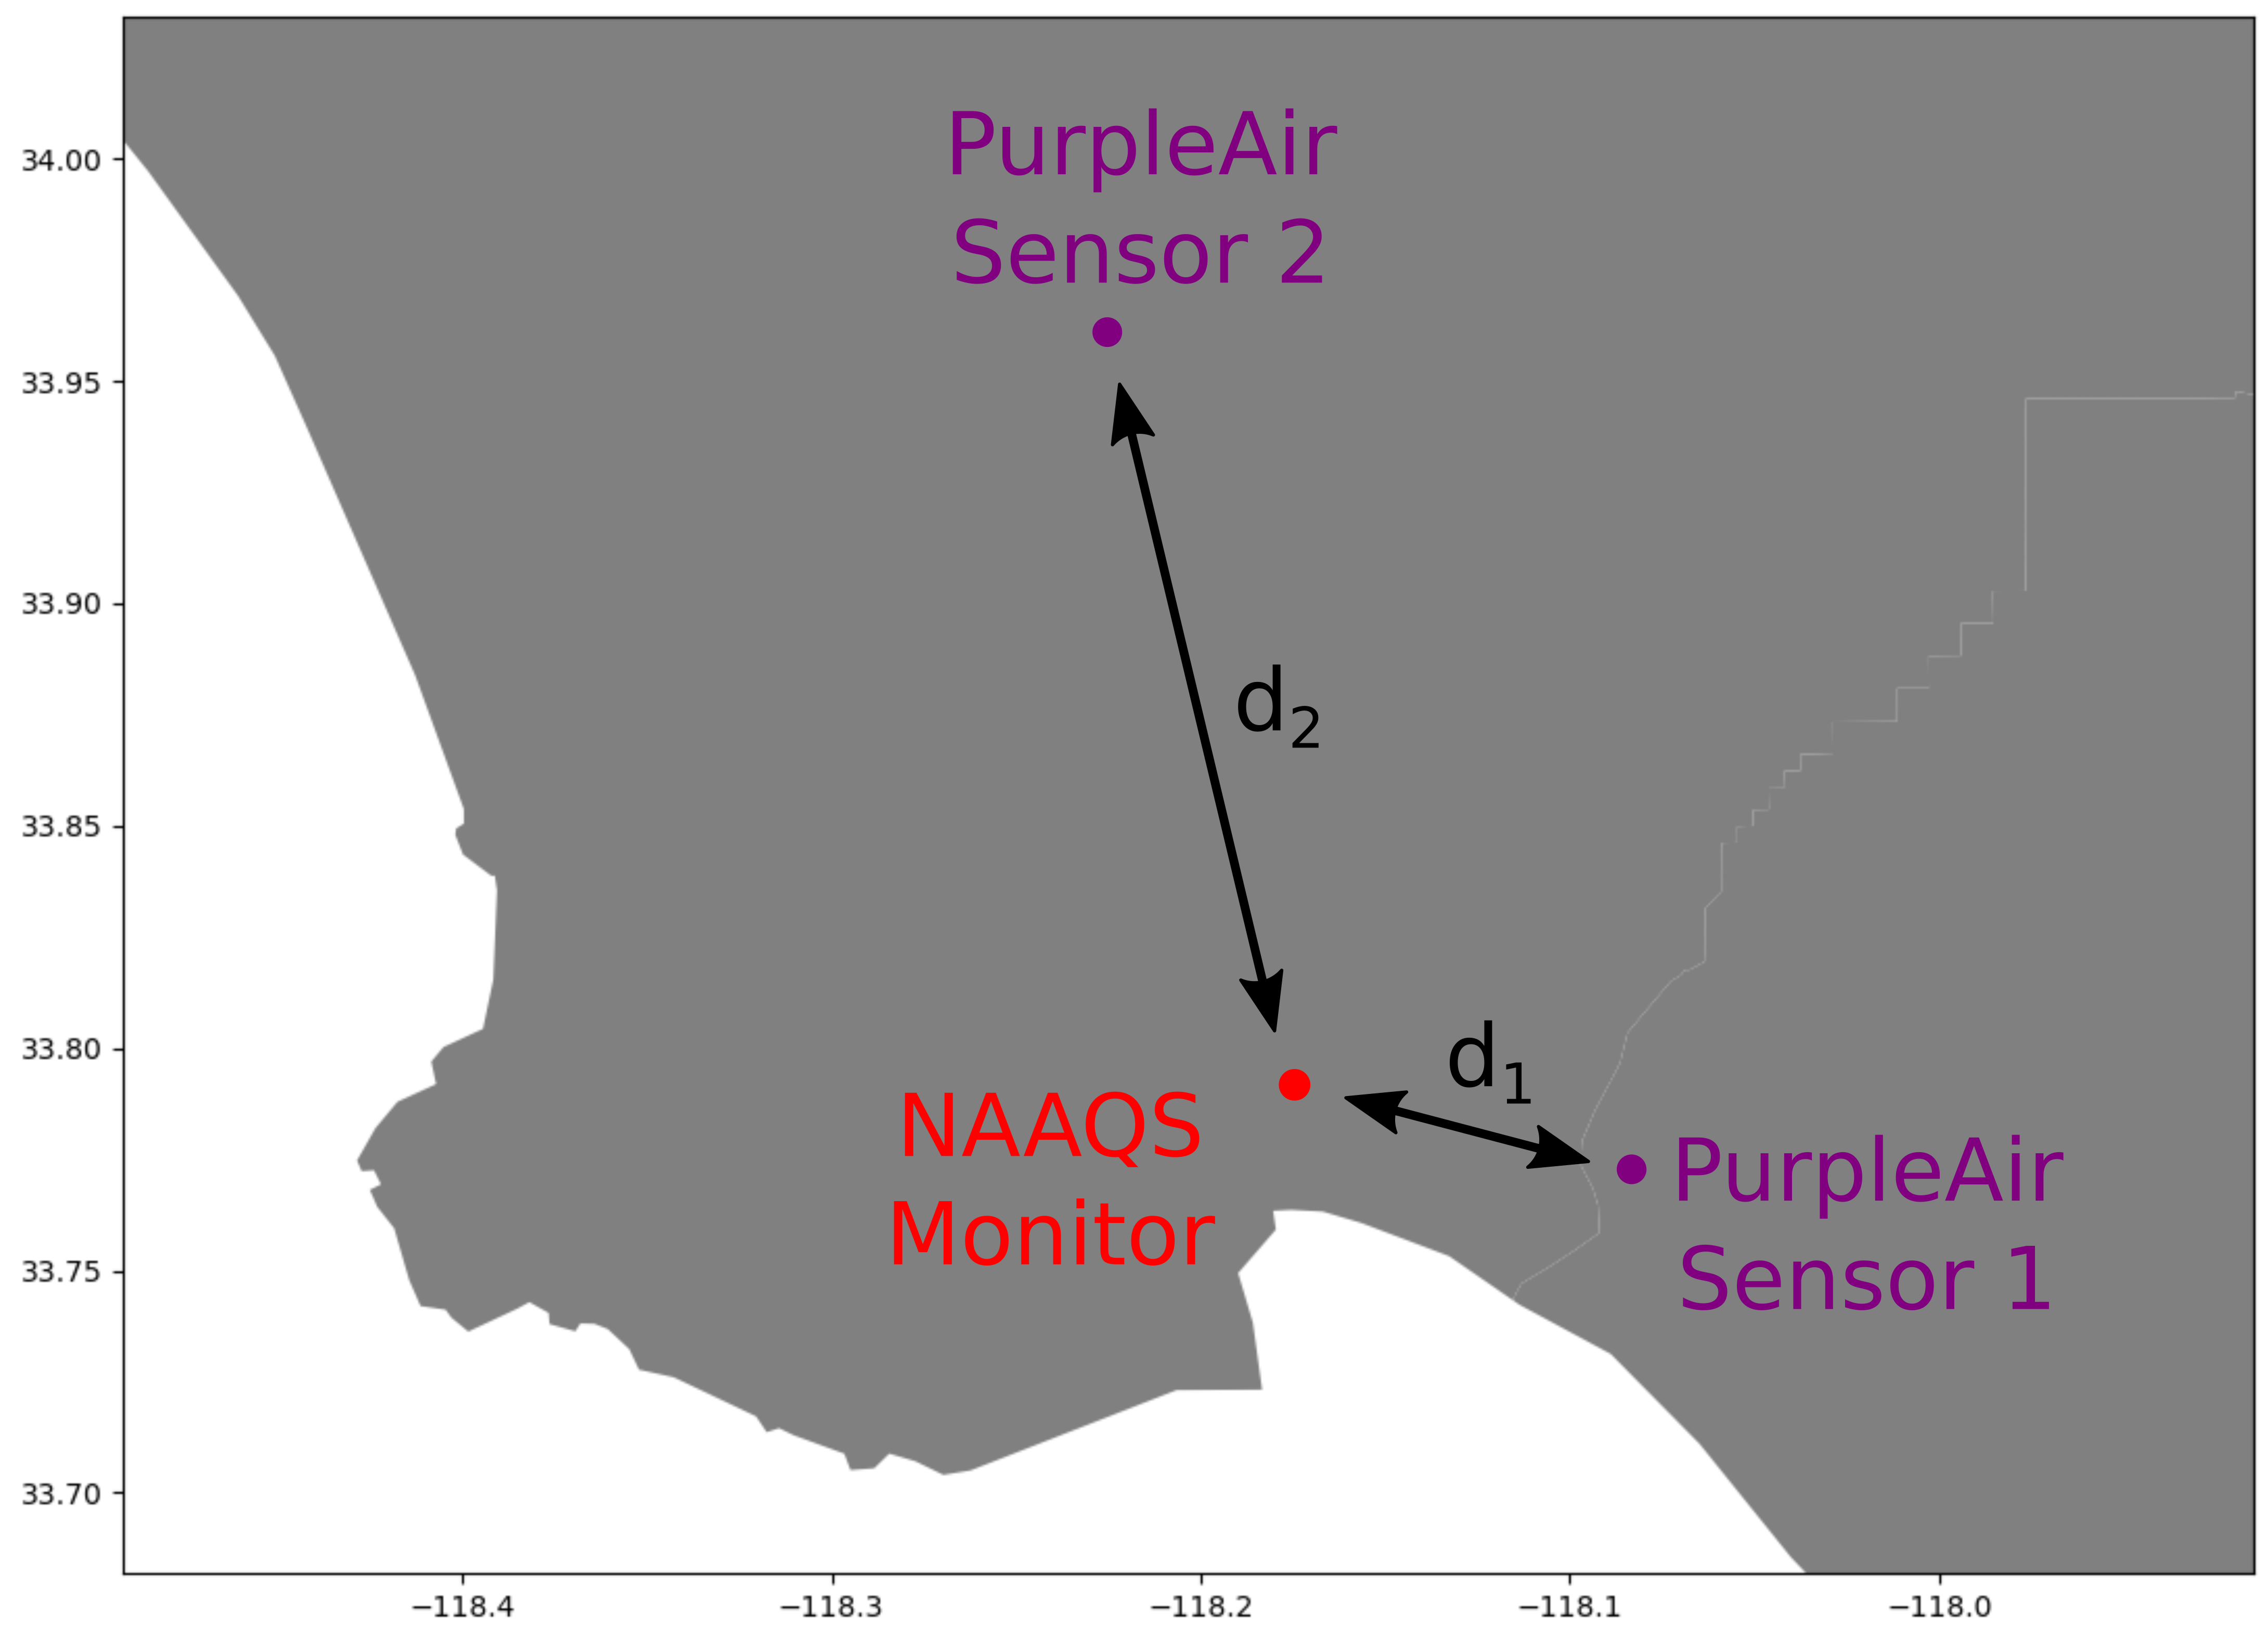
\includegraphics[width=0.5\textwidth]{output/figures/diagrams/IDW_diagram.png}
\\
\textbf{Inverse-distance Weighted Average Ambient PM2.5}

\begin{equation*}
    PA^{IDW}_t= \sum\limits_{j=1}^{J_t} \dfrac{\frac{1}{d_j}\cdot PA_{j,t}}{\sum\limits_j^{J_t}\frac{1}{d_j}}
    = \sum\limits_{j=1}^{J^t} w_{j,t}\cdot PA_{j,t}
\end{equation*}
\begin{itemize}
    \item $J_t$ = active PurpleAir sensors around the NAAQS monitor at time $t$
\end{itemize}

\end{frame}
%---------------------------------------------------------


%---------------------------------------------------------
%Predicting Missing EPA Data
\begin{frame}
\frametitle{Predicting Missing EPA Data}
\begin{equation*}
EPA_t = \beta_0 + \beta_1 PA^{IDW}_t + \varepsilon_t
\end{equation*}

\begin{table}[!htbp] \centering
  \caption{Reported NAAQS Monitor PM2.5 (site 037-4004)}
  \label{tab:reg_037-4004}
\begin{tabular}{@{\extracolsep{5pt}}lcc}
\\[-1.8ex]\hline
\hline \\[-1.8ex]
\\[-1.8ex] & (1) & (2) \\
\hline \\[-1.8ex]
 intercept & & 6.924$^{***}$ \\
  & & (0.076) \\
 PurpleAir IDW Average & 0.741$^{***}$ & 0.444$^{***}$ \\
  & (0.003) & (0.004) \\
\hline \\[-1.8ex]
 Observations & 36,813 & 36,813 \\
 $R^2$ & 0.658 & 0.240 \\
 F Statistic & 70924.412$^{***}$  & 11642.169$^{***}$  \\
\hline
\hline \\[-1.8ex]
& \multicolumn{2}{r}{$^{*}$p$<$0.1; $^{**}$p$<$0.05; $^{***}$p$<$0.01} \\
\end{tabular}
\end{table}
\end{frame}
%---------------------------------------------------------


%---------------------------------------------------------
%Design Values for an EPA site
\begin{frame}
\frametitle{Calculating Design Values for an EPA Site}
\end{frame}
%---------------------------------------------------------


%---------------------------------------------------------
%Results: Sample EPA Sites
\begin{frame}
\frametitle{Results: Sample EPA Sites}
\end{frame}
%---------------------------------------------------------


%---------------------------------------------------------
%Results: Fresno
\begin{frame}
\frametitle{Results: Fresno}
\end{frame}
%---------------------------------------------------------


%---------------------------------------------------------
%Conclusions & Discussion
\begin{frame}
\frametitle{Conclusions \& Discussion}
\end{frame}
%---------------------------------------------------------


%---------------------------------------------------------
%Future Work
\begin{frame}
\frametitle{Future Work}
\end{frame}
%---------------------------------------------------------


%---------------------------------------------------------
% Purple Air EPA Correction
\begin{frame}
\frametitle{Correction of PurpleAir Readings}
$$
\widetilde{PA}_{j,t}=\begin{cases}
			0.52*PA_{j,t} - 0.086*H_{j,t} + 5.75, & \text{if $PA_{j,t} \leq 343 \mu$g/m$^3$}\\
            0.46*PA_{j,t} + 0.(3.93e-4)PA_{j,t}^2 + 2.97, & \text{otherwise}
		 \end{cases}
$$
\begin{itemize}
    \item $PA_{j,t}$ = ambient PM2.5 measured by PurpleAir sensor $j$ at time $t$
    \item $H_{j,t}\in[0,1]$ is the relative humidity
\end{itemize}
\end{frame}
%---------------------------------------------------------


%---------------------------------------------------------
% Future Prediction Equation
\begin{frame}
\frametitle{Better Prediction of EPA PM2.5}

$$
\widetilde{PA}_{j,t}=\begin{cases}
			0.52*PA_{j,t} - 0.086*H_{j,t} + 5.75, & \text{if $PA_{j,t} \leq 343 \mu$g/m$^3$}\\
            0.46*PA_{j,t} + 0.(3.93e-4)PA_{j,t}^2 + 2.97, & \text{otherwise}
		 \end{cases}
$$
\begin{itemize}
    \item $PA_{j,t}$ = ambient PM2.5 measured by PurpleAir sensor $j$ at time $t$
    \item $H_{j,t}\in[0,1]$ is the relative humidity
\end{itemize}
\end{frame}
%---------------------------------------------------------


%---------------------------------------------------------
%Extra Tables
\begin{frame}
\frametitle{Table: }
\end{frame}
%---------------------------------------------------------












\end{document}




%    Examples

%%%%%%%%%%%%%%%%%% multi-slide text
\begin{frame}
In this slide \pause

the text will be partially visible \pause

And finally everything will be there
\end{frame}





%%%%%%%%%%%%%%%%%% highlighting text and theorem boxes
\begin{frame}
\frametitle{NAAQS Completeness Criteria}

In this slide, some important text will be
\alert{highlighted} because it's important.
Please, don't abuse it.

\begin{block}{Remark}
Sample text
\end{block}

\begin{alertblock}{Important theorem}
Sample text in red box
\end{alertblock}

\begin{examples}
Sample text in green box. The title of the block is ``Examples".
\end{examples}
\end{frame}








%Two columns
\begin{frame}
\frametitle{Two-column slide}

\begin{columns}

\column{0.5\textwidth}
This is a text in first column.
$$E=mc^2$$
\begin{itemize}
\item First item
\item Second item
\end{itemize}

\column{0.5\textwidth}
This text will be in the second column
and on a second tought this is a nice looking
layout in some cases.
\end{columns}
\end{frame}








